
%\documentclass[a4paper,twocolumn,psfig,subfigure,epsfig,fleqn,ausarbeitung,amssmb,float,caption,fontenc]{article}
\documentclass[a4paper,psfig,subfigure,epsfig,fleqn,ausarbeitung,amssmb,float,caption,fontenc]{article}
 
\pagestyle{empty}

\bibliographystyle{plain}

\usepackage{hyperref}
\usepackage{enumitem}
\usepackage{graphicx}

%set dimensions of columns, gap between columns, and paragraph indent

\setlength{\textheight}{24.7 cm}
\setlength{\columnsep}{1 cm}
\setlength{\textwidth}{16 cm}
%\setlength{\footheight}{0.0 cm}
\setlength{\topmargin}{0.0 cm}
\setlength{\headheight}{0.0 cm}
\setlength{\headsep}{-0.3 cm}
\setlength{\oddsidemargin}{0.0 cm}
\setlength{\parindent}{0.7 cm}
\setlength{\mathindent}{0mm}

% set page counter if document is part of proceedings
\setcounter{page}{23}
\renewcommand{\floatpagefraction}{0.9}
\renewcommand{\textfraction}{0.1}

%\renewcommand{\captionlabelfont}{\fontfamily{phv}\fontseries{bx}\fontsize{10}{10pt}\selectfont}
%\renewcommand{\captionfont}{\fontfamily{phv}\fontsize{10}{12pt}\selectfont}
%\setlength{\captionmargin}{0.5 cm}

\makeatletter
\makeatother
\def\RR{\hbox{I\kern-.2em\hbox{R}}}


\begin{document}

%don't want date printed
\date{}

%make title bold and 14 pt font (Latex default is non-bold, 16pt) 
\title{%~\\
%  ~\\
  \fontsize{14}{14pt} \bf Computer Vision Exercise Course I: Report}

\author{~\\
  ~\\
  \fontsize{12}{12pt}
  \begin{tabular}[t]{c c c}
  {\bf Alexander Cech}                    & {\bf Hamed Jafari-Sahamieh}             & {\bf Patrick Link}                      \\
  \small{Student of Visual Computing}     & \small{Student of Computer Science(?)}  & \small{Student of Computer Science(?)}  \\
  \small{Vienna University of Technology} & \small{Vienna University of Technology} & \small{Vienna University of Technology} \\
  \small{e08900070@student.tuwien.ac.at}  & \small{?}                               & \small{e11728332@student.tuwien.ac.at}  \\
  \end{tabular}
  ~\\ ~\\ ~\\
  \normalsize
  {\bf ABSTRACT} \\ 
  \noindent
  \hspace{0.2cm}
  \begin{minipage}[c]{15cm}
  \normalsize This is my abstract.  This is my abstract.  This is my
    abstract.  This is my abstract.  This is my abstract.  This is my
    abstract.  This is my abstract.  This is my abstract.  This is my
    abstract.  This is my abstract.  This is my abstract.  This is my
    abstract.\\
  \end{minipage}
%  ~\\ ~\\ ~\\
  \normalsize
%  {\bf KEYWORDS} \\ 
%  \normalsize
%  Keyword1, Keyword2, Keyword3, Keyword4, Keyword5, Keyword6.
  }

\maketitle

%I don't know why I have to reset thispagestyle, but otherwise get page numbers 
\normalfont
\thispagestyle{empty}

\section{Introduction}
\label{sec:introduction}


TODO and questions to ask:
\begin{itemize}[noitemsep]
\item Repeat theory and details of assignment sheet in the report?
\item Hamed is not signed up in TUWEL group?
\item Verify email addresses, affiliations.
\item Do we want an abstract and introduction?
\item Source code as appendix?
\item Index? List of figures?
\end{itemize}


This is a text to test the layout. This is a text to test the layout.
This is a text to test the layout.  This is a text to test the layout.
This is a text to test the layout. This is a text to test the layout.
This is a text to test the layout. This is a text to test the layout.
This is a text to test the layout.  This is a text to test the layout.
This is a text to test the layout. This is a text to test the layout.



This is a text to test the layout. This is a text to test the layout.
This is a text to test the layout.  This is a text to test the layout.
This is a text to test the layout. This is a text to test the layout.
This is a text to test the layout. This is a text to test the layout.
This is a text to test the layout.  This is a text to test the layou
This is a text to test the layout. This is a text to test the layout.
This is a text to test the layout.t. This is a text to test the
layout. This is a text to test the layout.  This is a text to test the
layout. This is a text to test the layout. This is a text to test the
layout.  This is a text to test the layout. This is a text to test the
layout. This is a text to test the layout.



This is a text to test the layout. This is a text to test the layout.
This is a text to test the layout.  This is a text to test the layout.
This is a text to test the layout. This is a text to test the layout.
This is a text to test the layout. This is a text to test the layout.
This is a text to test the layout.  This is a text to test the layout.
This is a text to test the layout. This is a text to test the layout.


\section{Assignment 1: Colorizing Images}
\label{sec:assignment1}

This is a text to test the layout. This is a text to test the layout.
This is a text to test the layout.  This is a text to test the layout.
This is a text to test the layout. This is a text to test the layout.
This is a text to test the layout. This is a text to test the layout.
This is a text to test the layout.  This is a text to test the layout.
This is a text to test the layout. This is a text to test the layout.
This is a text to test the layout. This is a text to test the layout.
This is a text to test the layout.

\subsection{Problem definition}

This is a text to test the layout. This is a text to test the layout.
This is a text to test the layout.  This is a text to test the layout.
This is a text to test the layout. This is a text to test the layout.
This is a text to test the layout. This is a text to test the layout.
This is a text to test the layout.  This is a text to test the layout.
This is a text to test the layout. This is a text to test the layout.

\subsection{Methodology}

This is a text to test the layout. This is a text to test the layout.
This is a text to test the layout.  This is a text to test the layout.
This is a text to test the layout. This is a text to test the layout.
This is a text to test the layout. This is a text to test the layout.
This is a text to test the layout.  This is a text to test the layout.
This is a text to test the layout. This is a text to test the layout.
This is a text to test the layout. This is a text to test the layout.
This is a text to test the layout.  This is a text to test the layout.
This is a text to test the layout. This is a text to test the layout.
This is a text to test the layout. This is a text to test the layout.
This is a text to test the layout.  This is a text to test the layout.
This is a text to test the layout. This is a text to test the layout.
This is a text to test the layout. This is a text to test the layout.
This is a text to test the layout.

\subsection{Experiments}

This is a text to test the layout. This is a text to test the layout.
This is a text to test the layout.  This is a text to test the layout.
This is a text to test the layout. This is a text to test the layout.
This is a text to test the layout. This is a text to test the layout.
This is a text to test the layout.  This is a text to test the layout.
This is a text to test the layout. This is a text to test the layout.
This is a text to test the layout. This is a text to test the layout.
This is a text to test the layout.  This is a text to test the layout.
This is a text to test the layout. This is a text to test the layout.
This is a text to test the layout. This is a text to test the layout.
This is a text to test the layout.  This is a text to test the layout.
This is a text to test the layout. This is a text to test the layout.
This is a text to test the layout. This is a text to test the layout.
This is a text to test the layout.

\subsection{Discussion}

This is a text to test the layout. This is a text to test the layout.
This is a text to test the layout.  This is a text to test the layout.
This is a text to test the layout. This is a text to test the layout.

This is a text to test the layout.  This is a text to test the layout.
This is a text to test the layout. This is a text to test the layout.
This is a text to test the layout. This is a text to test the layout.
This is a text to test the layout.  This is a text to test the layout.

% -----------------------------------------------------------------------------------------------

\section{Assignment 2: Image Segmentation by \texorpdfstring{$K$}-means Clustering}
\label{sec:assignment2}

This is a text to test the layout.

\subsection{Problem definition}

This is a text to test the layout.

\subsection{Methodology}

This is a text to test the layout.

\subsection{Experiments}

This is a text to test the layout.

\subsection{Discussion}

This is a text to test the layout.

% -----------------------------------------------------------------------------------------------

\section{Assignment 3: Scale-Invariant Blob Detection}
\label{sec:assignment3}

This assignment is about locating blobs of different sizes in images. A Laplacian blob detector is implemented and used in a scale-invariant way by convolving it with repeatedly blurred versions of the image to be analyzed.

\subsection{Problem definition}

Given an image, the problem is to find blob-like features of varying scale. In specific, the goals are to:
\begin{itemize}[noitemsep]
\item Implement a Laplacian of Gaussian (LoG) blob detector
\item Apply it to a reference image (\texttt{butterfly.jpg}) and an image of choice. Also apply it to half-sized versions of the images
\item Indicate the found blobs by overlaying circles, with the circle radii being representative of the found blob's size
\item Plot the LoG response over all scales at a specific keypoint for both the original and half-sized image
\item Discuss the results
\end{itemize}

\subsection{Methodology}

Todo ...

\subsection{Experiments}

Todo ...

\begin{figure}[h]
	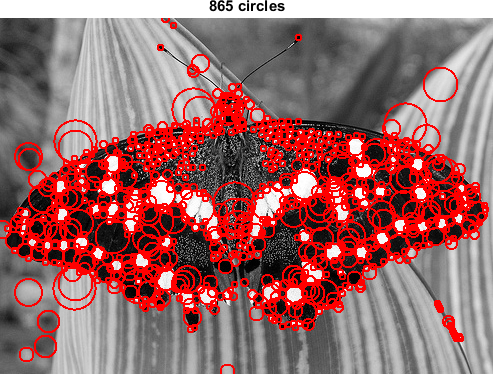
\includegraphics[width=0.5\textwidth]{figures/a3_butterfly_k015.png}
	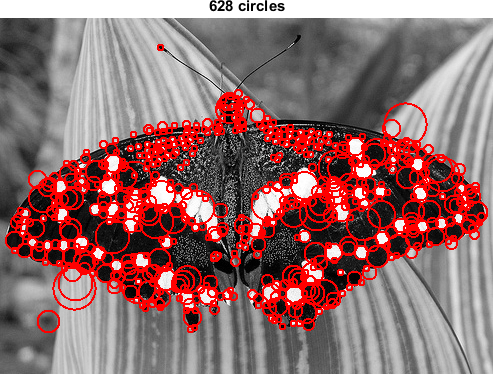
\includegraphics[width=0.5\textwidth]{figures/a3_butterfly_k018.png}
	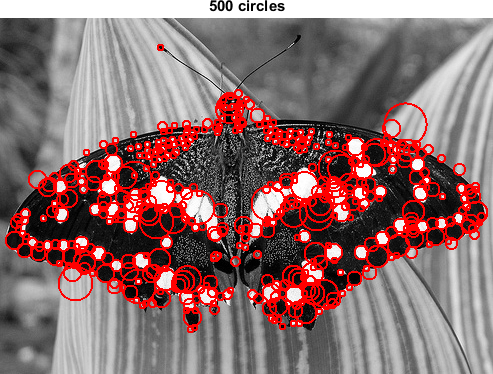
\includegraphics[width=0.5\textwidth]{figures/a3_butterfly_k020.png}
	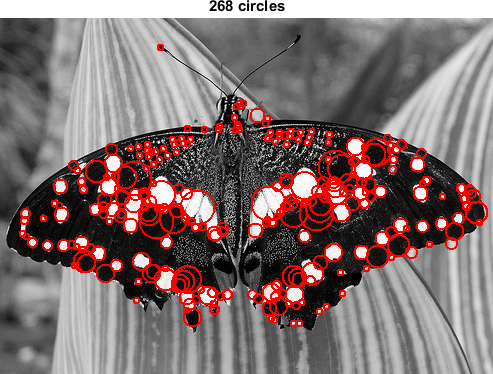
\includegraphics[width=0.5\textwidth]{figures/a3_butterfly_k025.png}
	\caption{Illustration of the effect of different thresholds $k$. Top left: $k=0.15$. Top right: $k=0.18$. Bottom left: $k=0.20$. Bottom right: $k=0.25$.}
	\label{fig:a3:thresholds}
\end{figure}

\begin{figure}[h]
	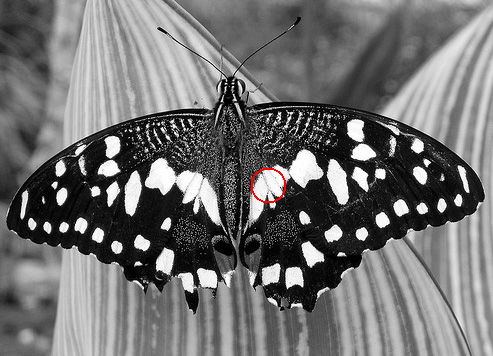
\includegraphics[width=0.5\textwidth]{figures/a3_butterfly_keypoint.png}
	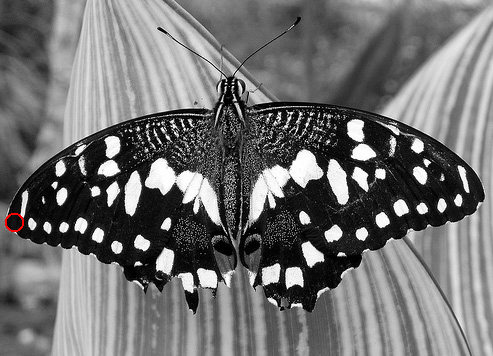
\includegraphics[width=0.5\textwidth]{figures/a3_butterfly_keypoint_2.png}
	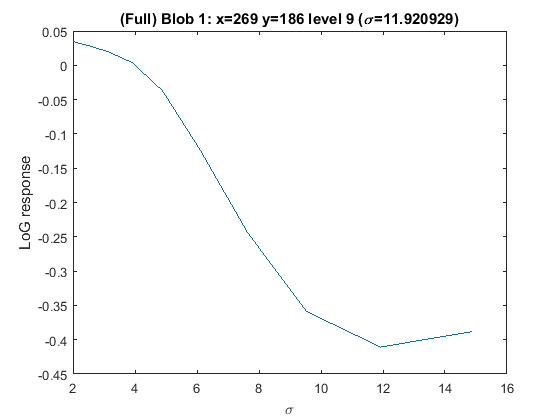
\includegraphics[width=0.5\textwidth]{figures/a3_butterfly_log_full.png}
	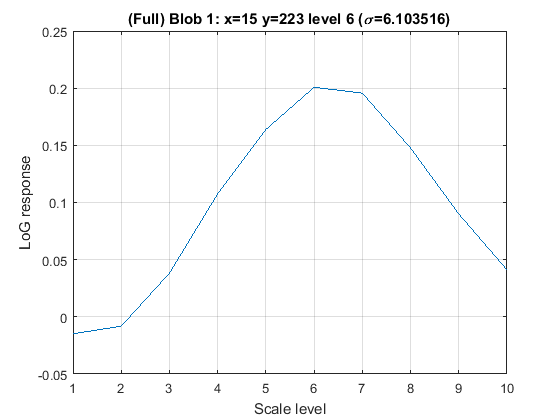
\includegraphics[width=0.5\textwidth]{figures/a3_butterfly_log_full_2.png}
	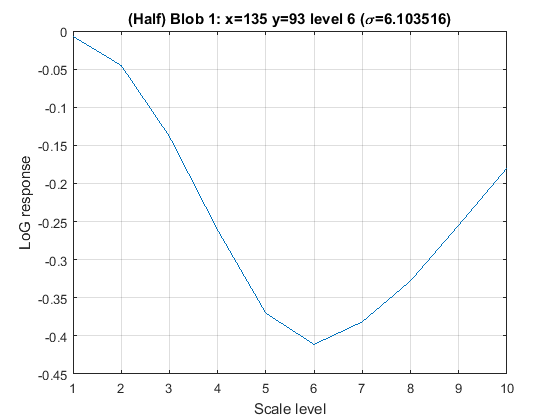
\includegraphics[width=0.5\textwidth]{figures/a3_butterfly_log_half.png}
	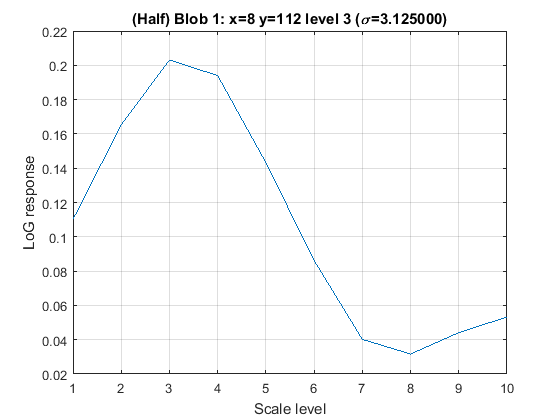
\includegraphics[width=0.5\textwidth]{figures/a3_butterfly_log_half_2.png}
	\caption{LoG response for two selected keypoints. The top row shows the chosen keypoint, the second and third rows show the LoG response for the full-sized and half-sized image. Left: A white-on-black blob (negative LoG response), right: a black-on-white blob (positive LoG response).}
	\label{fig:a3:logresponse}
\end{figure}


\subsection{Discussion}

Todo ...

% -----------------------------------------
% Appendix for source code ?
\appendix
\section{Source code}
\subsection{Implemention of Assignment 1}
\subsection{Implemention of Assignment 2}
\subsection{Implemention of Assignment 3}


%% *********
%% Bibliography
%% *********

\fontsize{9}{10pt}
\bibliographystyle{plain}

\begin{thebibliography}{10}

% uncomment/add used references

\bibitem{Szeliski}
{\bf R.~Szeliski},
\newblock \textit{Computer Vision: Algorithms and Applications},
\newblock Springer, 2010.
\newblock \url{http://szeliski.org/Book/drafts/SzeliskiBook_20100903_draft.pdf}.

\end{thebibliography}

\end{document}

%%% Local Variables: 
%%% mode: latex
%%% TeX-master: t
%%% End: 

